% This version of CVPR template is provided by Ming-Ming Cheng.
% Please leave an issue if you found a bug:
% https://github.com/MCG-NKU/CVPR_Template.

%\documentclass[review]{cvpr}
\documentclass[final]{cvpr}

\usepackage{times}
\usepackage{epsfig}
\usepackage{graphicx}
\usepackage{amsmath}
\usepackage{amssymb}

% Include other packages here, before hyperref.

% If you comment hyperref and then uncomment it, you should delete
% egpaper.aux before re-running latex.  (Or just hit 'q' on the first latex
% run, let it finish, and you should be clear).
\usepackage[pagebackref=true,breaklinks=true,colorlinks,bookmarks=false]{hyperref}


\def\cvprPaperID{****} % *** Enter the CVPR Paper ID here
\def\confYear{CVPR 2021}
%\setcounter{page}{4321} % For final version only


\begin{document}

%%%%%%%%% TITLE
\title{Comparing GANs with RNNs on Predicting Commodity Prices}

\author{Quinn Murphey\\
University of Texas at San Antonio\\
1 UTSA Circle San Antonio, TX\\
{\tt\small quinn.murphey@my.utsa.edu}
% For a paper whose authors are all at the same institution,
% omit the following lines up until the closing ``}''.
% Additional authors and addresses can be added with ``\and'',
% just like the second author.
% To save space, use either the email address or home page, not both
\and
Adrian Ramos\\
University of Texas at San Antonio\\
1 UTSA Circle San Antonio, TX\\
{\tt\small adrian.ramos@my.utsa.edu}

\and
Gabriel Soliz\\
University of Texas at San Antonio\\
1 UTSA Circle San Antonio, TX\\
{\tt\small gabriel.soliz@my.utsa.edu}
}

\maketitle


%%%%%%%%% ABSTRACT
\begin{abstract}
    The ability to accurately project the price of commodities is one of the
    most useful applications of deep learning. It finds use from hedge funds
    seeking to maximize profit to public administrations modelling the outcomes
    of different policies. In the typical year, these algorithms are quite 
    successful, at least more so than their human counterparts. However, these
    models have almost always failed to predict drastic economic downturns such
    as the crash of oil in 2020 or the now expected crashes of Bitcoin.
    It’s critical to everyone that we can prepare for sudden events that can
    drastically alter the markets. Building off of the work of Tang et al.
    \cite{tang}, we use historical commodity prices along with Google
    search trends and news report sentimentatlity to hopefully achieve better
    commodity price predictions both in normal and abnormal times. In order
    to accomplish this task, we will use a combination of different deep
    learning algorithms including RNNs, CNNs, and GANs. We will compare our
    results with those from similar papers.
\end{abstract}

%%%%%%%%% BODY TEXT
%~~~~~~~~~~~~~~~~~~~~~~~~~~~~~~~~~~~~~~~~~~~~~~~~~~~~~~~~~~~~~~~~~~~~~~~~~~~~~~~
\section{Introduction}

    The price fluctuation of good and stocks are often difficult to predict due to
    the numerous amounts of variables that play an important role of the price
    function. While there exists research that reflects on those expected variables
    \cite{romero}. Additionally, the research conducted which compares multiple results
    comprised from other researchers and their unique test leading to their results
    \cite{srivastava}.  The importance of being able to accurately predict the price of
    commodities is vital to creating plans to aid those in need. The more accurate
    our forecasting ability is, the better prepared we can hope to be in uncertain
    times. It would allow emergency services and first responders to allocate enough
    supplies in the event of unpredictable events that could cause server damage to
    our infrastructure.  However, there has been minimal research on the price
    fluctuation of goods and stocks due to external events, such as war, pandemics,
    or environmental catastrophes. While reports have been brought up that show
    certain effects of specific tragedies, such as the COVID-19 pandemic report
    \cite{mead}. The rate that prices fluctuate of goods and stocks during times of
    crisis and compared to other times of crisis could potentially help uncover
    areas which are most impacted. Including opportunities for potential preventive
    measures to attempt to thwart a severe effect.

    The source code for our project can be found at 
    \url{https://www.github.org/Nragis/cs4263-project}.

%~~~~~~~~~~~~~~~~~~~~~~~~~~~~~~~~~~~~~~~~~~~~~~~~~~~~~~~~~~~~~~~~~~~~~~~~~~~~~~~
\section{Related Work}

    From what we have observed there seems to be certain trends when trying to
    predict natural gas prices. The trend majority of the articles such as
    “Forecasting Natural Gas Spot Prices with Machine Learning” use is by taking
    the price of the gas as far as you have a data set for and then using
    adaptive and regression models to predict the gas prices future. The next
    theme that some articles use such as “Deep Neural Network Model for
    Improving Price Prediction of Natural Gas” is that they look at the current
    trend of natural gas and other similar items on something like google and if
    there is a trend of natural gas possibly becoming volatile with other
    forecasts also coming to this conclusion then it changes the prediction
    accordingly. The least common way that I have found is one explored in the
    paper “Natural Gas Price Prediction with Big Data” where the authors use
    sentiment analysis on a large body of literature, most commonly the news.
    This way while uncommon is surprisingly effective with it being able to tell
    the sentiment within the text and according to how drastic it is it changes
    the predictions.

%~~~~~~~~~~~~~~~~~~~~~~~~~~~~~~~~~~~~~~~~~~~~~~~~~~~~~~~~~~~~~~~~~~~~~~~~~~~~~~~
\section{Proposed Approach}

    For this project we will approach it in our own unique way. We will utilize the
    Energy Information Agency's Natural Gas dataset spanning the past several
    years. We will also utilize a time-series regression algorithm to analyze and
    predict the price for natural gas. Using a time-series regression algorithm
    should help us with utilizing and processing the data set we have chosen to its
    fullest extent utilizing every bit of knowledge we have to give an accurate
    prediction not only of the past but also the future. Utilizing this method our
    prediction data should be superior to the traditional econometric models and
    have the ability to predict future data points.

%~~~~~~~~~~~~~~~~~~~~~~~~~~~~~~~~~~~~~~~~~~~~~~~~~~~~~~~~~~~~~~~~~~~~~~~~~~~~~~~
\section{Data}

\subsection{Commodity Prices}

    To be able to compare directly with Tang et al. \cite{tang}, we will use the
    same daily NYMEX natural gas futures prices from the US Energy Information
    Administration website (\url{https://www.eia.gov/}). These futures are for 1
    month, 2 month, 3 month, and 4 month time periods. In alignment with Tang,
    we will be using data from these four contracts from January 2013 to June
    2019. 1,638 records in total.

    In future updates, we will have more papers with different types of
    commodities, specifically those not related to energy. Until we get better
    results with the NYMEX dataset, we will not be working with other data.

\subsection{Internet Search History}

    We will be using Google Trends (\url{https://trends.google.com/}) as our source for Google search history data.
    In this paper, we will be using the daily search for the respective
    commodity: natural gas, [COMMODITY2], and [COMMODITY3] and a few recession
    related terms such as [RECESSION\_TERMS] each covering the exact time period
    of the commodity price dataset. These datasets are 2,372, [BLANK], and [BLANK]
    records long for natural gas, [COMMODITY2], and [COMMODITY3] respectively.

\subsection{News Report Sentimentality}

    We collected the title and bodytext of all news articles from Yahoo Finance
    (We want to experiment with different news sources, both financial and not,
    and both credible and not) with the keyword natural gas, [COMMODITY2], and 
    [COMMODITY3] respectively, each covering the exact time period of the
    commodity price dataset. We do not have an exact length for this dataset due
    to still deciding which news sites to use.

%~~~~~~~~~~~~~~~~~~~~~~~~~~~~~~~~~~~~~~~~~~~~~~~~~~~~~~~~~~~~~~~~~~~~~~~~~~~~~~~
\section{Experiments}

    In alignment with Tang, we will use mean absolute error (MAE) and root mean
    square error (RMSE) to compare results. Our goal is to minimize these
    values, indicating a more accurate regression.

    \begin{equation}
        MAE = \frac{1}{N}\sum_i^N|y_i - \hat{y_i}| \\
    \end{equation}

    \begin{equation}
        RMSE = \sqrt{\frac{1}{N}\sum_i^N(y_i - \hat{y_i})^2}
    \end{equation}

    Where $y_i$ and $\hat{y_i}$ are the real and predicted values respectively.

%~~~~~~~~~~~~~~~~~~~~~~~~~~~~~~~~~~~~~~~~~~~~~~~~~~~~~~~~~~~~~~~~~~~~~~~~~~~~~~~
\section{Results}

    Note: Our results relate to a prior direction of our paper, meaning they do not
    use the same datasets as we mention above.

    Using the World Economic Overview dataset published by the International
    Monetary Fund semi-annually which tracks 44 economic indicators including
    Gross Domestic Product (GDP), Gross Domestic Product per Capita (GDPPC), and
    Average Consumer Prices Inflation Index (PCPI) for 194 countries from 1980
    to 2020. While the database isn't completely full, most of the entries of
    the 8820 row, 57 column dataset are filled.

    After which, we turn the dataset into a multivariable (each indicator) time
    series for each country. We then pass a 10 width window over each time
    series, creating a data set of 6208 rows - each with a country, 396 input
    variables (44 indicators across 9 years) and one output variable: the tenth
    year value of GDPPC (in purchasing power).

    We then split the dataset into a 0.8, 0.1, 0.1 split for training,
    validation, and test datasets.

    We compared four basic models to each other:
    \begin{enumerate}
        \item Linear: A simple matrix multiplication represented by a single layer,
            single perceptron neural network.

        \item Single-Layer Perceptron: A single layer of 512 neurons with ReLU
            acivation functions.

        \item Multi-Layer Perceptron: Two layers of 512 neurons with ReLU
            activation functions

        \item CNN Without Pooling: Three 1D convolutional layers with 3 length
            kernels and 256, 128, and 64 filters respectively followed by one
            layer of 256 ReLU perceptrons.
    \end{enumerate}

    Our results were as follows:

    \begin{center}

        {\small 
            TABLE 1: COMPARISON OF GDPPC PREDICTION RESULTS ACROSS DIFFERENT MODELS
        }

        \begin{tabular}{||c c||}
             \hline
             Model & MAE\\ [0.5ex]
             \hline\hline
             Linear &  379.37 \\
             \hline
             Single & 20.31 \\
             \hline
             Multi & 19.74 \\
             \hline
             CNN & 16.00 \\
             \hline
        \end{tabular}
        
        \vspace{24pt}

        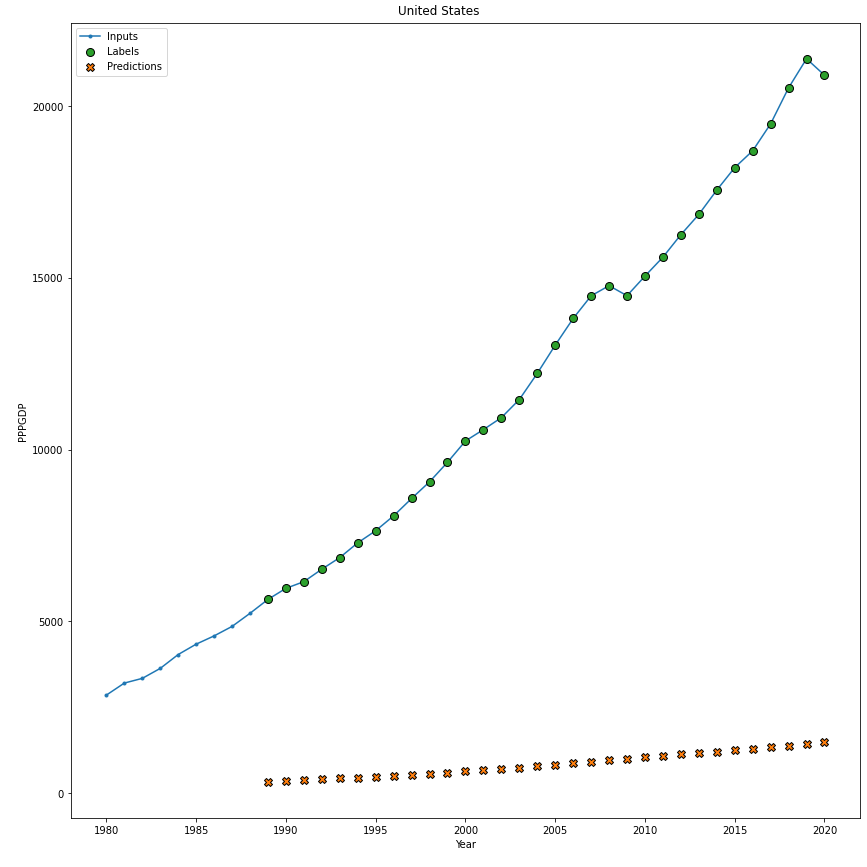
\includegraphics[scale=0.27]{linearFiller.png}
        {\small
            FIGURE 2: LINEAR MODEL PREDICTIONS OF GDPPC
        }

        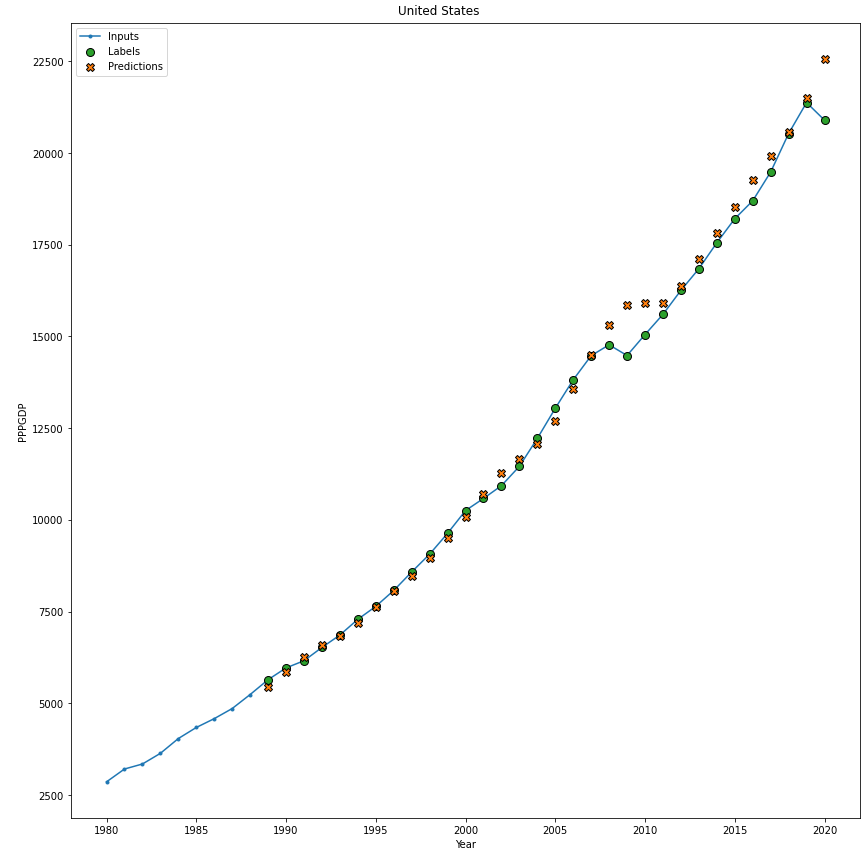
\includegraphics[scale=0.27]{singleFiller.png}
        {\small
            FIGURE 3: SINGLE-LAYER PERCEPTRON MODEL PREDICTIONS OF GDPPC
        }

        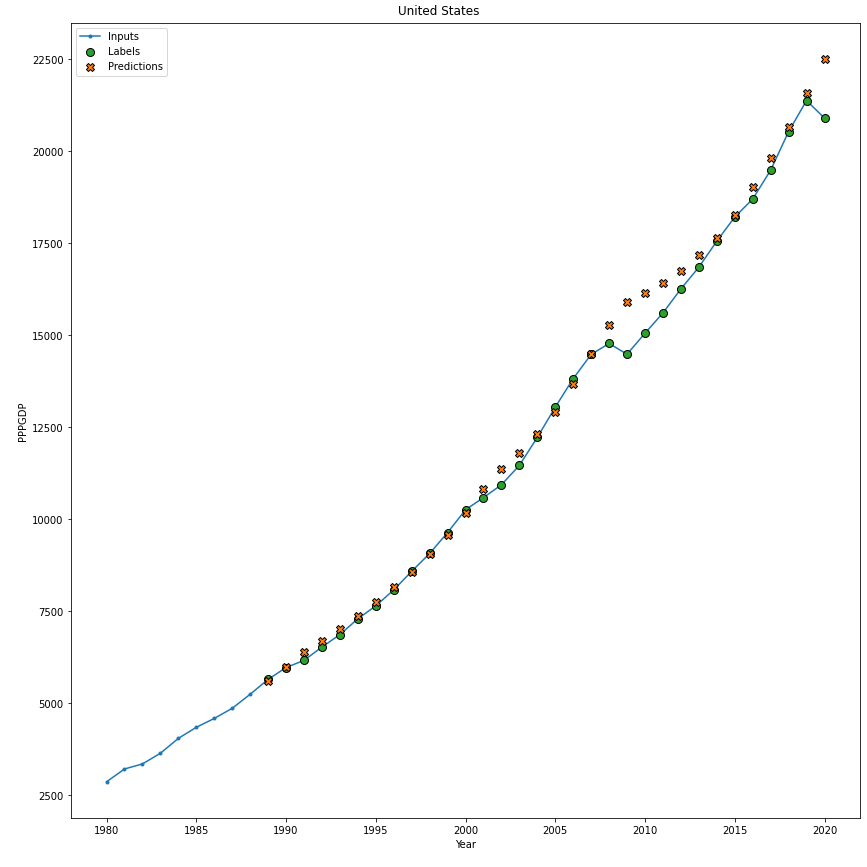
\includegraphics[scale=0.27]{multiFiller.png}
        {\small
            FIGURE 4: MULTI-LAYER PERCEPTRON MODEL PREDICTIONS OF GDPPC
        }

        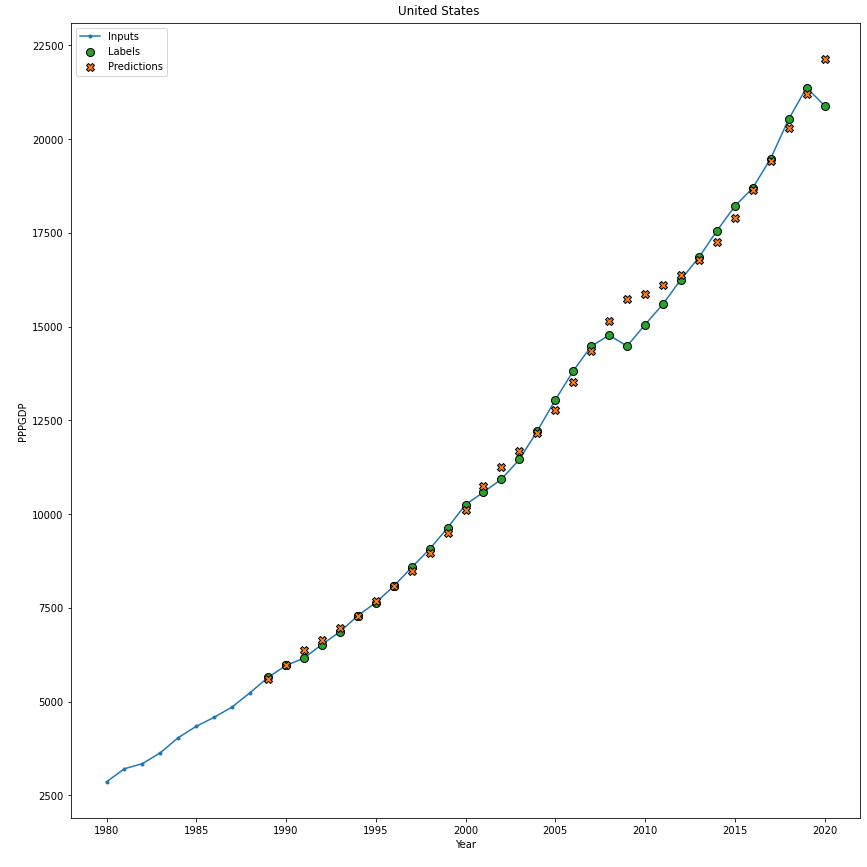
\includegraphics[scale=0.27]{CNNFiller.png}
        {\small
            FIGURE 5: CNN WITHOUT POOLING MODEL PREDICTIONS OF GDPPC
        }
    \end{center}



%~~~~~~~~~~~~~~~~~~~~~~~~~~~~~~~~~~~~~~~~~~~~~~~~~~~~~~~~~~~~~~~~~~~~~~~~~~~~~~~
\section{Conclusion}

We will write this section once we have final results.

\nocite{*}

{\small
    \bibliographystyle{ieee_fullname}
    \bibliography{egbib}
}

\end{document}
